\documentclass[spanish,12pt]{article}
\usepackage[T1]{fontenc}
\usepackage[utf8]{inputenc}
\usepackage{amsmath}
\usepackage{stackrel}
\usepackage{graphicx}
\usepackage{epstopdf}
\usepackage{subcaption}
\makeatletter
%%%%%%%%%%%%%%%%%%%%%%%%%%%%%% User specified LaTeX commands.
\usepackage{algorithm}
\usepackage{algorithmic}
\floatname{algorithm}{Algoritmo}
\renewcommand{\listalgorithmname}{Lista de algoritmos}
\renewcommand{\algorithmicrequire}{\textbf{Entrada:}}
\renewcommand{\algorithmicensure}{\textbf{Salida:}}
\renewcommand{\algorithmicend}{\textbf{fin}}
\renewcommand{\algorithmicif}{\textbf{si}}
\renewcommand{\algorithmicthen}{\textbf{entonces}}
\renewcommand{\algorithmicelse}{\textbf{si no}}
\renewcommand{\algorithmicelsif}{\algorithmicelse,\ \algorithmicif}
\renewcommand{\algorithmicendif}{\algorithmicend\ \algorithmicif}
\renewcommand{\algorithmicfor}{\textbf{para}}
\renewcommand{\algorithmicforall}{\textbf{para todo}}
\renewcommand{\algorithmicdo}{\textbf{hacer}}
\renewcommand{\algorithmicendfor}{\algorithmicend\ \algorithmicfor}
\renewcommand{\algorithmicwhile}{\textbf{mientras}}
\renewcommand{\algorithmicendwhile}{\algorithmicend\ \algorithmicwhile}
\renewcommand{\algorithmicloop}{\textbf{repetir}}
\renewcommand{\algorithmicendloop}{\algorithmicend\ \algorithmicloop}
\renewcommand{\algorithmicrepeat}{\textbf{repetir}}
\renewcommand{\algorithmicuntil}{\textbf{hasta que}}
\renewcommand{\algorithmicprint}{\textbf{imprimir}} 
\renewcommand{\algorithmicreturn}{\textbf{devolver}} 
\renewcommand{\algorithmictrue}{\textbf{cierto }} 
\renewcommand{\algorithmicfalse}{\textbf{falso }} 

\usepackage{verbatim}
\usepackage{mathpazo}
\usepackage{blindtext}
\usepackage{multirow}
\usepackage{booktabs}
%\usepackage{array}
\usepackage{numprint}
\npdecimalsign{.}
\nprounddigits{2}

% horizontal margins: 1.0 + 6.5 + 1.0 = 8.5
\setlength{\oddsidemargin}{0.0in}
\setlength{\textwidth}{6.5in}
% vertical margins: 1.0 + 9.0 + 1.0 = 11.0
\setlength{\topmargin}{0.0in}
\setlength{\headheight}{12pt}
\setlength{\headsep}{13pt}
\setlength{\textheight}{625pt}
\setlength{\footskip}{24pt}

\renewcommand{\textfraction}{0.10}
\renewcommand{\topfraction}{0.85}
\renewcommand{\bottomfraction}{0.85}
\renewcommand{\floatpagefraction}{0.90}
\renewcommand{\baselinestretch}{1.2}
\usepackage{caption}
\captionsetup[table]{name=Tabla}
\date{}

\makeatother

\usepackage{babel}
\addto\shorthandsspanish{\spanishdeactivate{~<>.}}

\begin{document}
\begin{center}
\huge{LTI Cinvestav}\\[16pt]

\includegraphics[scale=0.08]{imagenes/cinvestav2.jpg}\\[1pt]
\large{\textbf{Máquinas de soporte vectorial con \emph{kernels}}}\\[16pt]
\textbf{Reconocimiento de patrones}\\[6pt]
Profesor: Dr. Wilfrido Gómez Flores \\[16pt]
Estudiante: Rafael Pérez Torres\\[16pt]
\par\end{center}


\section{Introducción}

Las máquinas de soporte vectorial son clasificadores basados en la
idea de máximo margen entre dos líneas (hiperplanos) que separan a
instancias de dos clases. Dichos hiperplanos son conocidos como vectores
de soporte, que mientras mayor margen describan disminuirán el riesgo
de que un patrón desconocido sea clasificado de forma incorrecta,
alcanzando así la generalización del clasificador.

Las máquinas de soporte vectorial, como cualquier clasificador lineal,
pueden intentar la clasificación de datos linealmente no separables,
a través de una función kernel. Dicha función realiza una transformación
de los datos en un espacio de baja dimensionalidad a otro de alta
dimensionalidad en el que sea posible alcanzar esta separabilidad.

El presente documento muestra los resultados de la implementación
de el clasificador de máquinas de soporte vectorial utilizando distintas
funciones kernel con diferentes parámetros para las etapa de entrenamiento.

\section{Marco teórico}

Las máquinas de soporte vectorial atienden a un problema específico
que otro tipo de clasificadores lineales, como el perceptrón y sus
variantes dejan de lado: dado un conjunto de clases (linealmente o
no separables) existe más de un hiperplano que puede definir la separación
entre las mismas; sin embargo, no todos los hiperplanos ofrecen la
misma calidad o margen de separación entre las clases.

En ese sentido, la idea general en las máquinas de soporte vectorial
es identificar aquel hiperplano que ofrece el mayor margen de separación
entre las instancias de las diferentes clases. 

Para identificar el mejor hiperplano, este clasificador busca aquellos
datos (vectores) que se encuentren más hacia el margen \emph{interno}
de las clases. Si se consideran dos clases, se tendrían dos vectores
delimitando a cada una de las dos clases. Dichos vectores son llamados
vectores de soporte, ya que en ellos la máquina se basa para obtener
el hiperplano que esté justo a la mitad, y que a la postre será el
hiperplano que ofrezca la mayor separabilidad entre las clases, como
se muestra en la Figura \ref{fig:Identificacion-de-vectores}.

\begin{figure}
\begin{centering}
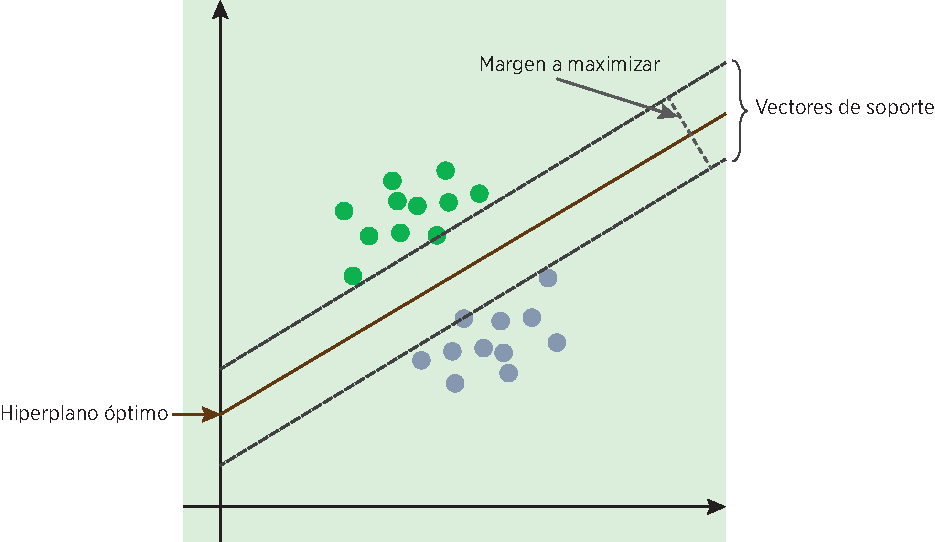
\includegraphics{imagenes/svm}
\par\end{centering}
\protect\caption{Identificación de vectores de soporte e hiperplano óptimo.\label{fig:Identificacion-de-vectores}}
\end{figure}

\section{Metodología}

La actividad consistió en realizar el conjunto de pasos descrito en el Algoritmo \ref{alg:algoritmo-svm} para realizar el entrenamiento y la clasificación utilizando las máquinas de soporte vectorial.
\begin{algorithm} 
\begin{algorithmic}[1] 
\STATE Crear matriz Hessiana $H = Ytr_i,Ytr_j,K(Xtr_i,Xtr_j)$
\STATE Encontrar $\alpha$, tal que 
$\underset{\alpha}{max\left[\stackrel[i=1]{N}{\sum}\alpha_{i}-\frac{1}{2}\alpha^{T}H\alpha\right]} \text{sujeto a}~ 0\leq \alpha_{i}\leq{C} ~\forall i ~\text{y}\sum_{i=1}^{N}\alpha_{i}y_{i}=0$
\STATE Determinar los vectores de soporte $\left\{x_{s},y_{s} \right\}$ que satisfacen la condición $ 0 < \alpha_{i} <  {C} $.
\STATE Calcular el bias:
$w_{0}=\frac{1}{N_s}\sum_{s\in S}\left\{ y_s - \sum_{m\in S}\alpha_m y_m K(x_m , x_s) \right\}$
\STATE Dado un patrón $x'$, se clasificará según:
$y' = \text{sign}\left\{ K(x_s , x')^{T} \alpha_s y_s + w_0 \right\}$
\end{algorithmic} 
\caption{Algoritmo para la clasificación con \emph{SVM}} 
\label{alg:algoritmo-svm}
\end{algorithm}


Se realizó la división de cada dataset en 70\% para entrenamiento y 30\% para prueba.
Asimismo, se preparó la secuencia de parámetros mostrada en la Tabla \ref{tbl:parametros} para la implementación de las funciones kernel lineal ($K(x_i, x_j) = x^T_i x_j$), polinomial ($K(x_i, x_j) = (x^T_i x_j)^2$) y \emph{rbf} ($K(x_i, x_j)=\text{exp}(-\gamma \left\lVert x_i - x_j \right\rVert_2^2$) para cada uno de los cuatro datasets considerados en la asignación: \emph{BreastMG, BreastUS, Diabetes} y \emph{Heart}.

\begin{table}[h]
\centering
\begin{tabular}{@{}ccl@{}}
\toprule
\multicolumn{1}{c}{\textbf{Función kernel}} & \multicolumn{1}{c}{\textbf{Parámetro}} & \multicolumn{1}{c}{\textbf{Valores}} \\ \midrule
Lineal                                      & C                                      & 1, 10, 100, 1000                     \\ \cmidrule{2-3}
\multirow{2}{*}{Polinomial}                 & Orden                                  & 2, 5, 10, 100                        \\
                                            & C                                      & 1, 10, 100, 1000                     \\ \cmidrule{2-3}
\multirow{2}{*}{RBF}                        & Gamma                                  & 0.01, 0.1, 0.5, 1.0                  \\
                                            & C                                      & 1, 10, 100, 1000                     \\ \bottomrule
\end{tabular}
\caption{Configuración de parámetros para la ejecución de las \emph{SVM}}
\label{tbl:parametros}
\end{table}

Respecto a la utilización de estos parámetros, se realizaron 31 experimentos con cada combinación de los parámetros.
Por ejemplo, para la función kernel polinomial se ejecutaron 31 repeticiones con la tupla (orden, C) = (2,1), 31 repeticiones con la tupla (2,10), etcétera.

\section{Resultados obtenidos}
La ejecución del algoritmo para clasificación mediante \emph{SVM} se realizó, como ha sido mencionado, 31 veces por cada configuración de parámetros para la función kernel sobre los cuatro datasets proporcionados. 
A continuación se describen los resultados obtenidos por cada tipo de función kernel aplicada.

La Tabla \ref{tbl:kernel-lineal-error} muestra los porcentajes de error obtenidos por ls \emph{SVM} utilizando una función kernel lineal.
Puede observarse que el parámetro $C=10$ obtuvo los porcentajes de error más bajos para todos los datasets, a excepción del \emph{BreastMG}.
En general, a través de esta función se obtuvieron porcentajes de error no mayores al 25\%.

La Tabla \ref{tbl:kernel-lineal-time} muestra los tiempos de ejecución del kernel lineal por las 31 ejecuciones para cada uno de los datasets.
No puede inferirse información relevante, salvo que el dataset de \emph{Diabetes} es el que mayor tiempo toma para su procesamiento (contiene 768 muestras de 8 dimensiones), mientras que el dataset \emph{Heart} es el más rápido en procesarse (contiene 270 muestras de 13 dimensiones).

\begin{table}[h]
\centering
\scriptsize
\begin{tabular}{@{}ccccc@{}}
\toprule
\textbf{\begin{tabular}[c]{@{}c@{}}Dataset /\\  Parameter (C)\end{tabular}} & \textbf{BreastMG} & \textbf{BreastUS} & \textbf{Diabetes} & \textbf{Heart} \\ \midrule
1                                                                           & 2.3719                & 10.396                & 24.165                & 17.483             \\
10                                                                          & 3.3397                & 9.3794                & 24.109                & 17.324             \\
100                                                                         & 7.4194                & 10.396                & 24.727                & 18.041             \\
1000                                                                        & 8.425                 & 15.954                & 25.512                & 19.833             \\ \bottomrule
\end{tabular}
\caption{Porcentajes de error del kernel lineal.}
\label{tbl:kernel-lineal-error}
\end{table}

\begin{table}[h]
\centering
\scriptsize
\begin{tabular}{@{}ccccc@{}}
\toprule
\textbf{\begin{tabular}[c]{@{}c@{}}Dataset/\\ Parameter(C)\end{tabular}} & \textbf{BreastMG} & \textbf{BreastUS} & \textbf{Diabetes} & \textbf{Heart} \\ \midrule
1                                                                        & 119.79            & 139.26            & 215.88            & 24.785         \\
10                                                                       & 121.53            & 145.6             & 219.14            & 25.098         \\
100                                                                      & 117.92            & 155.8             & 222.78            & 24.979         \\
1000                                                                     & 118.78            & 156.31            & 211.97            & 23.287         \\ \bottomrule
\end{tabular}
\caption{Tiempos de ejecución (segundos) del kernel lineal.}
\label{tbl:kernel-lineal-time}
\end{table}

En adelante, por cuestiones de espacio, solamente se muestran las gráficas de los resultados para las funciones kernel polinomial y \emph{rbf}.
La Figura \ref{fig:polinomial-error} muestra los porcentajes de errores obtenidos por la función kernel polinomial con distintas configuraciones.
De dicha figura puede concluirse que para estos datasets, la \emph{SVM} con una función kernel polinomial con dimensiones bajas tiende a obtener porcentajes de error menores.
En general, sus porcentajes de error son no mayores a 64.77\%.
De la Figura \ref{fig:polinomial-time}, que muestra los tiempos de ejecución para esta misma función kernel, puede observarse que la duración de la ejecución es casi duplicada a comparación de la función kernel lineal.

\begin{figure}
        \centering
        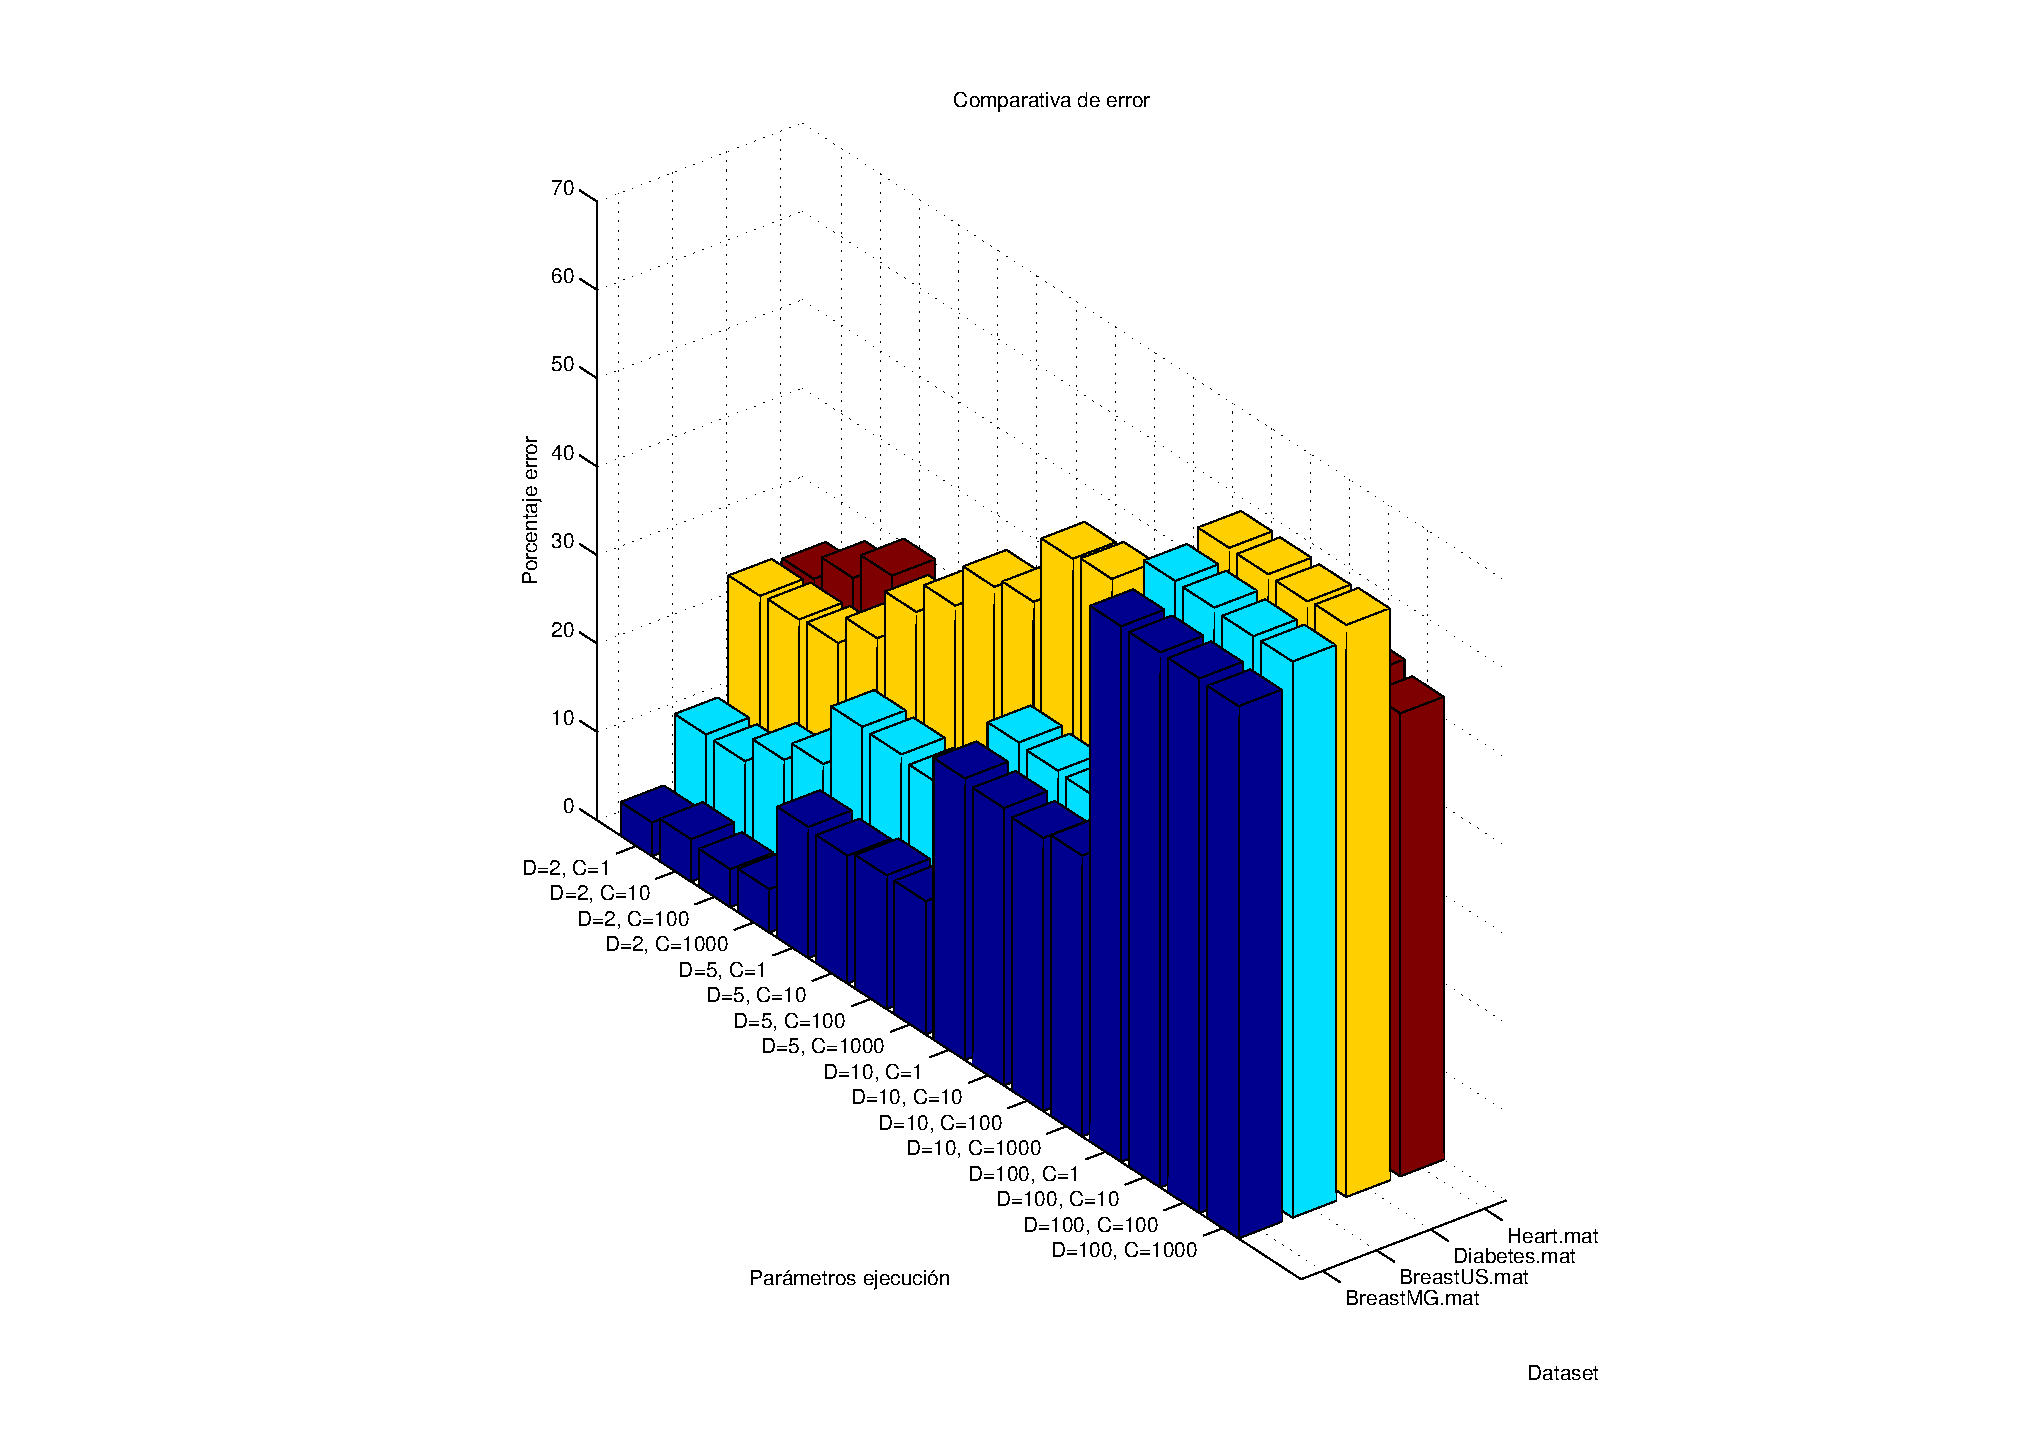
\includegraphics[width=\textwidth]{imagenes/polinomial-error}
        \caption{Porcentajes de error obtenidos por la función kernel polinomial.}\label{fig:polinomial-error}
\end{figure}


\begin{figure}
        \centering
        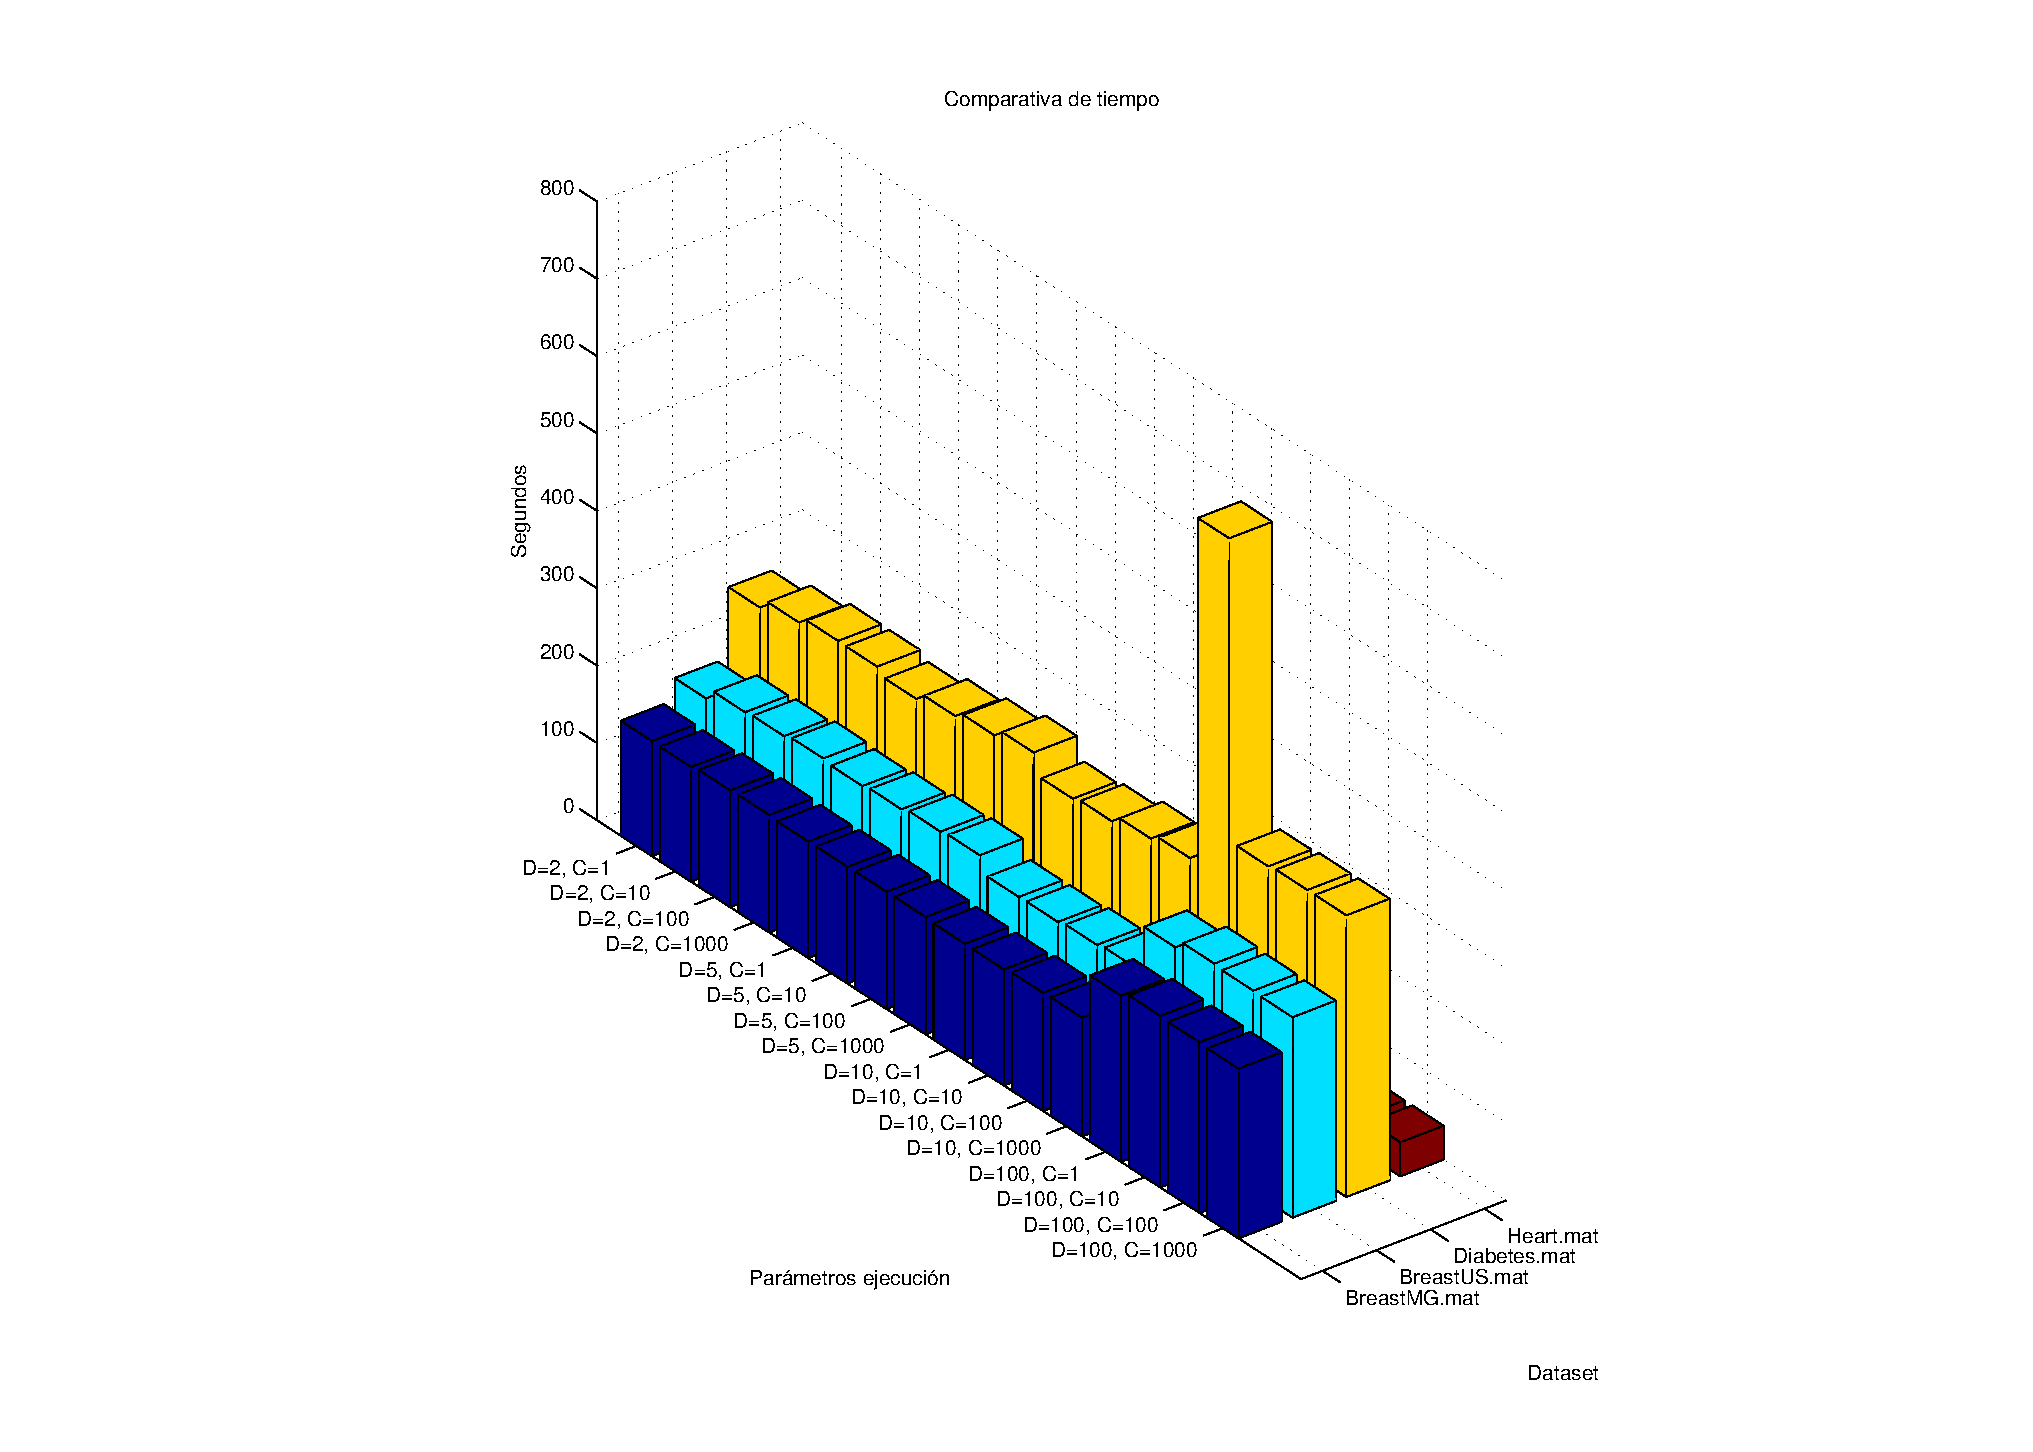
\includegraphics[width=\textwidth]{imagenes/polinomial-time}
        \caption{Tiempos de ejecución obtenidos por la función kernel polinomial.}\label{fig:polinomial-time}
\end{figure}

% \begin{figure}
%         \centering
%         \begin{subfigure}[b]{0.7\textwidth}
%                 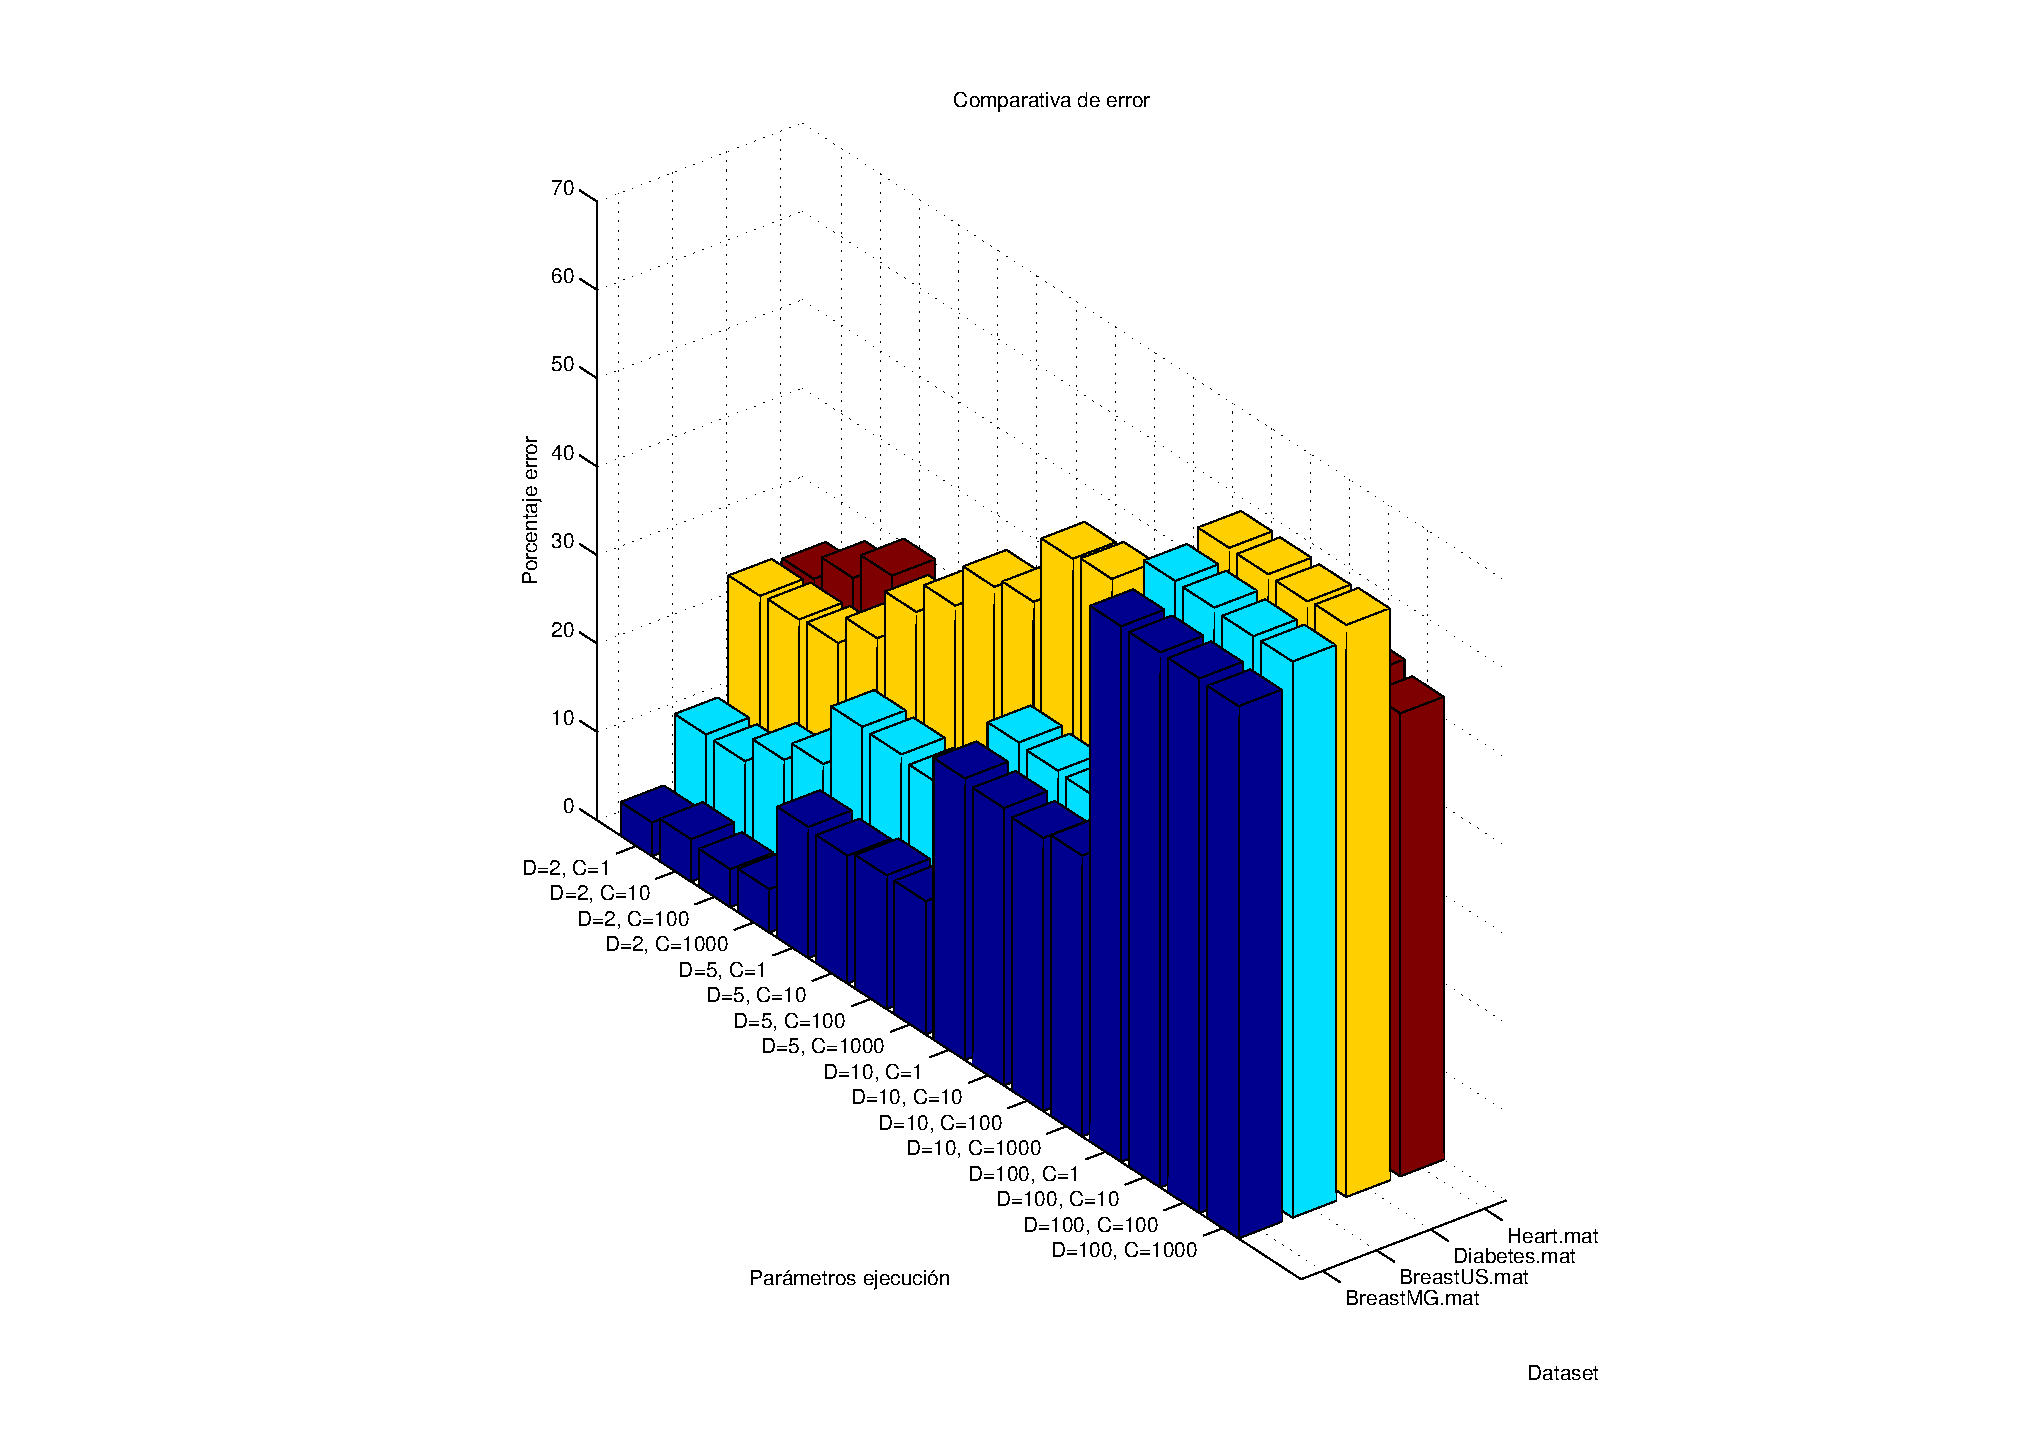
\includegraphics[width=\textwidth]{imagenes/polinomial-error}
%                 \caption{A gull}
%                 \label{fig:gull}
%         \end{subfigure}%
%         ~ %add desired spacing between images, e. g. ~, \quad, \qquad, \hfill etc.
%           %(or a blank line to force the subfigure onto a new line)
%         \begin{subfigure}[b]{0.7\textwidth}
%                 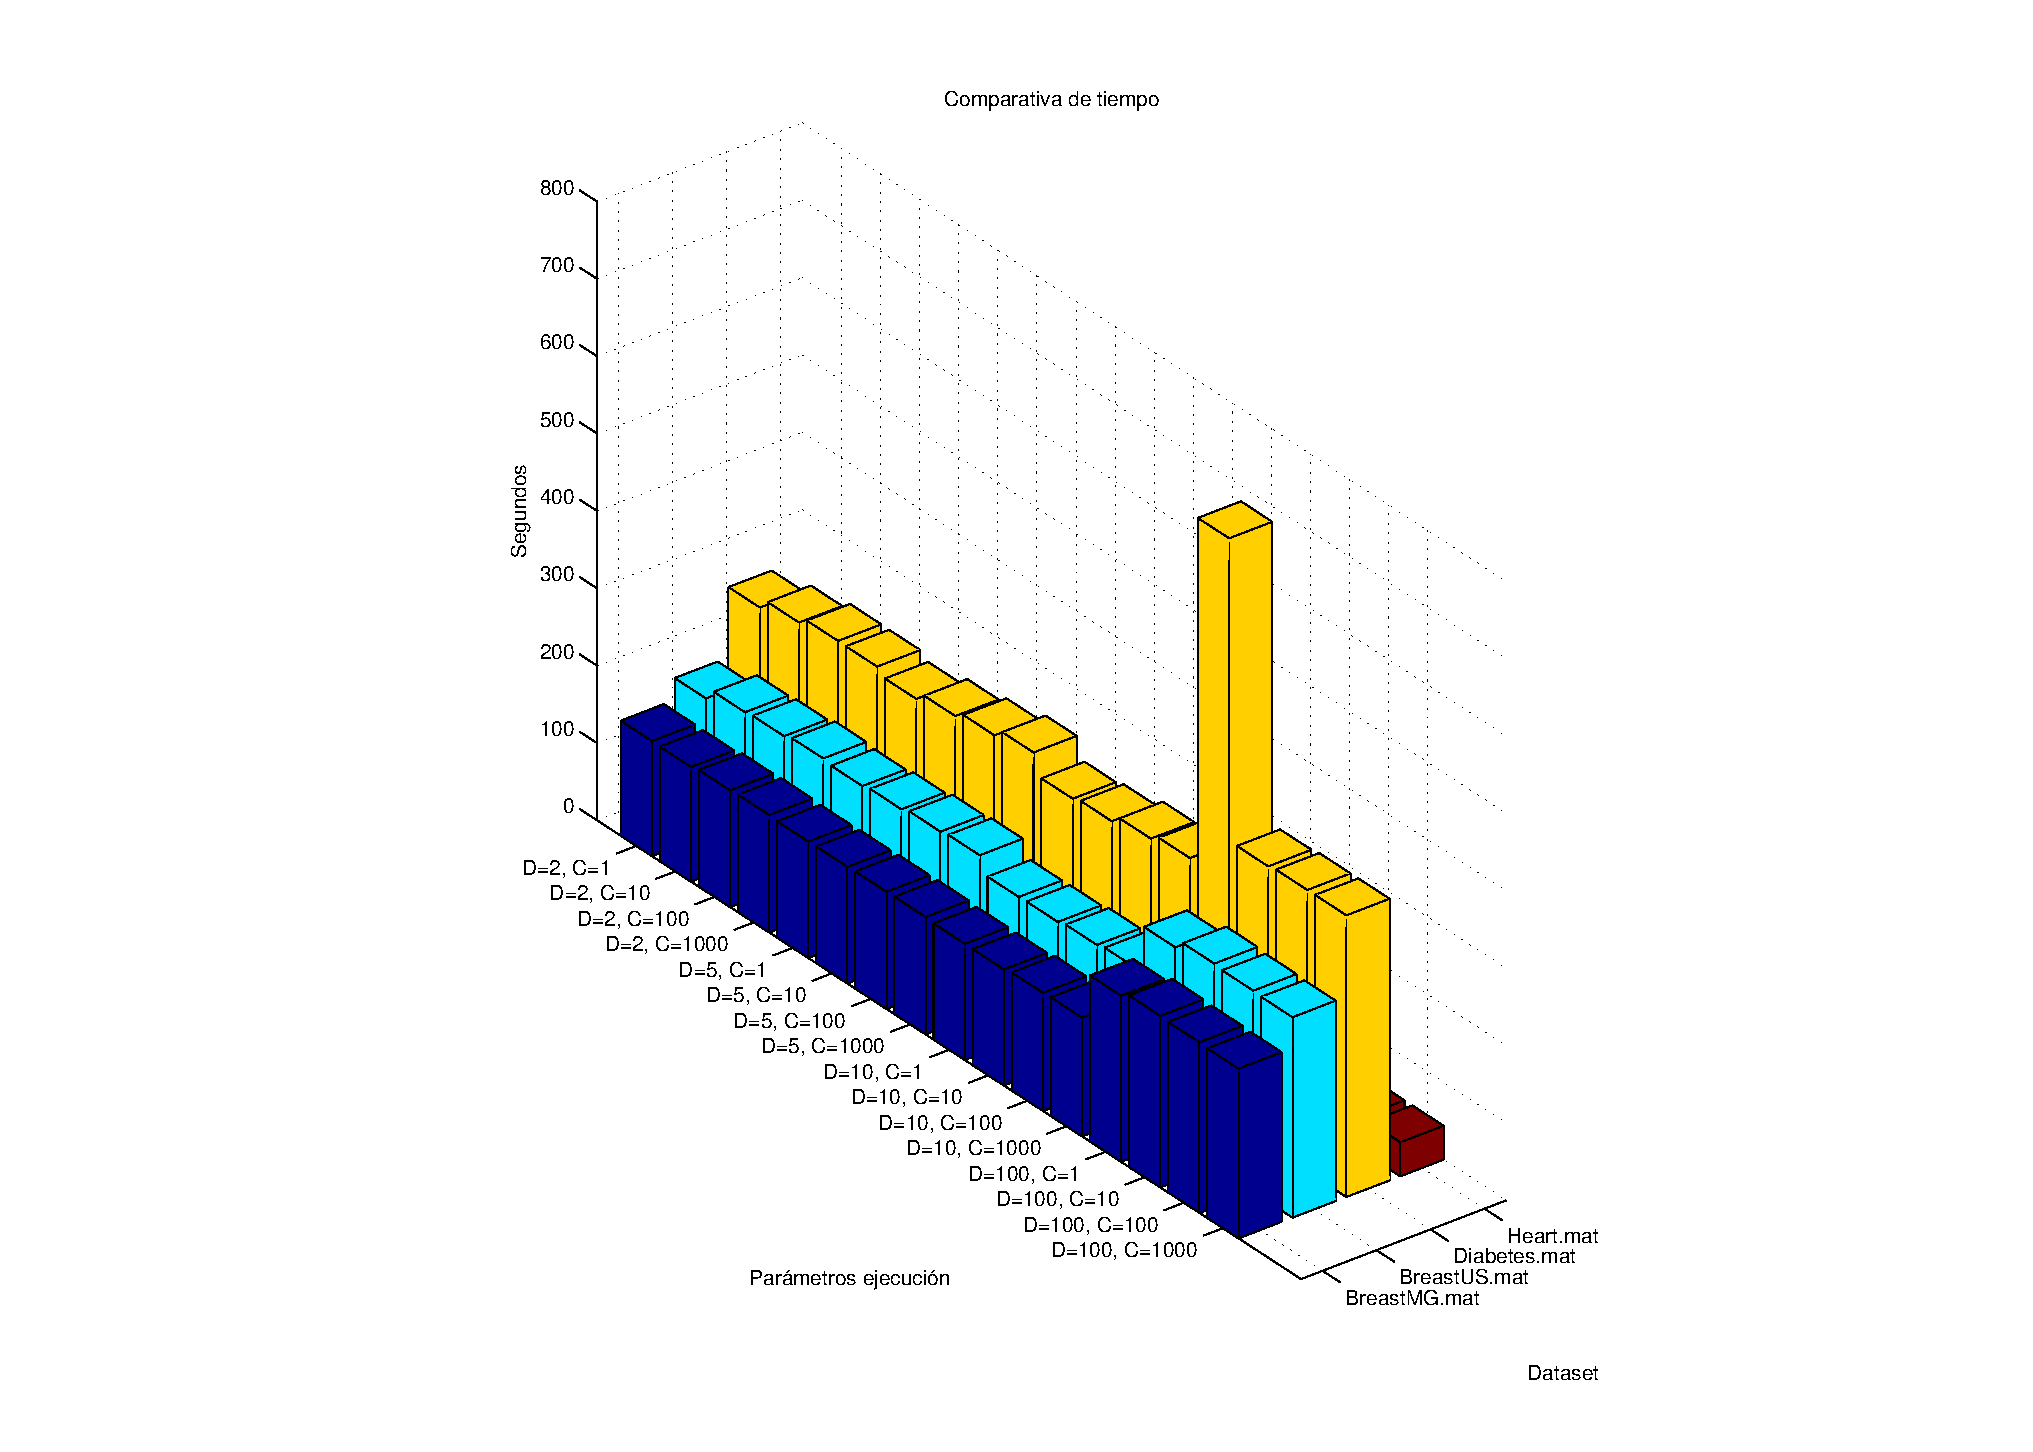
\includegraphics[width=\textwidth]{imagenes/polinomial-time}
%                 \caption{A tiger}
%                 \label{fig:tiger}
%         \end{subfigure}
%         \caption{Pictures of animals}\label{fig:animals}
% \end{figure}


En la Figura \ref{fig:rbf-error} se muestran los porcentajes de error de la función kernel \emph{rbf} con las distintas configuraciones implementadas.
Puede notarse que ofrece los mejores resultados para el dataset \emph{BreastMG}.
En general, sus porcentajes de error son no mayores a 33.28\%.
Asimismo, la Figura \ref{fig:rbf-time} muestra los tiempos de ejecución para este tipo de función.
Puede observarse que la clasificación a través de esta función kernel es la que mayor tiempo requiere.
\begin{figure}
        \centering
        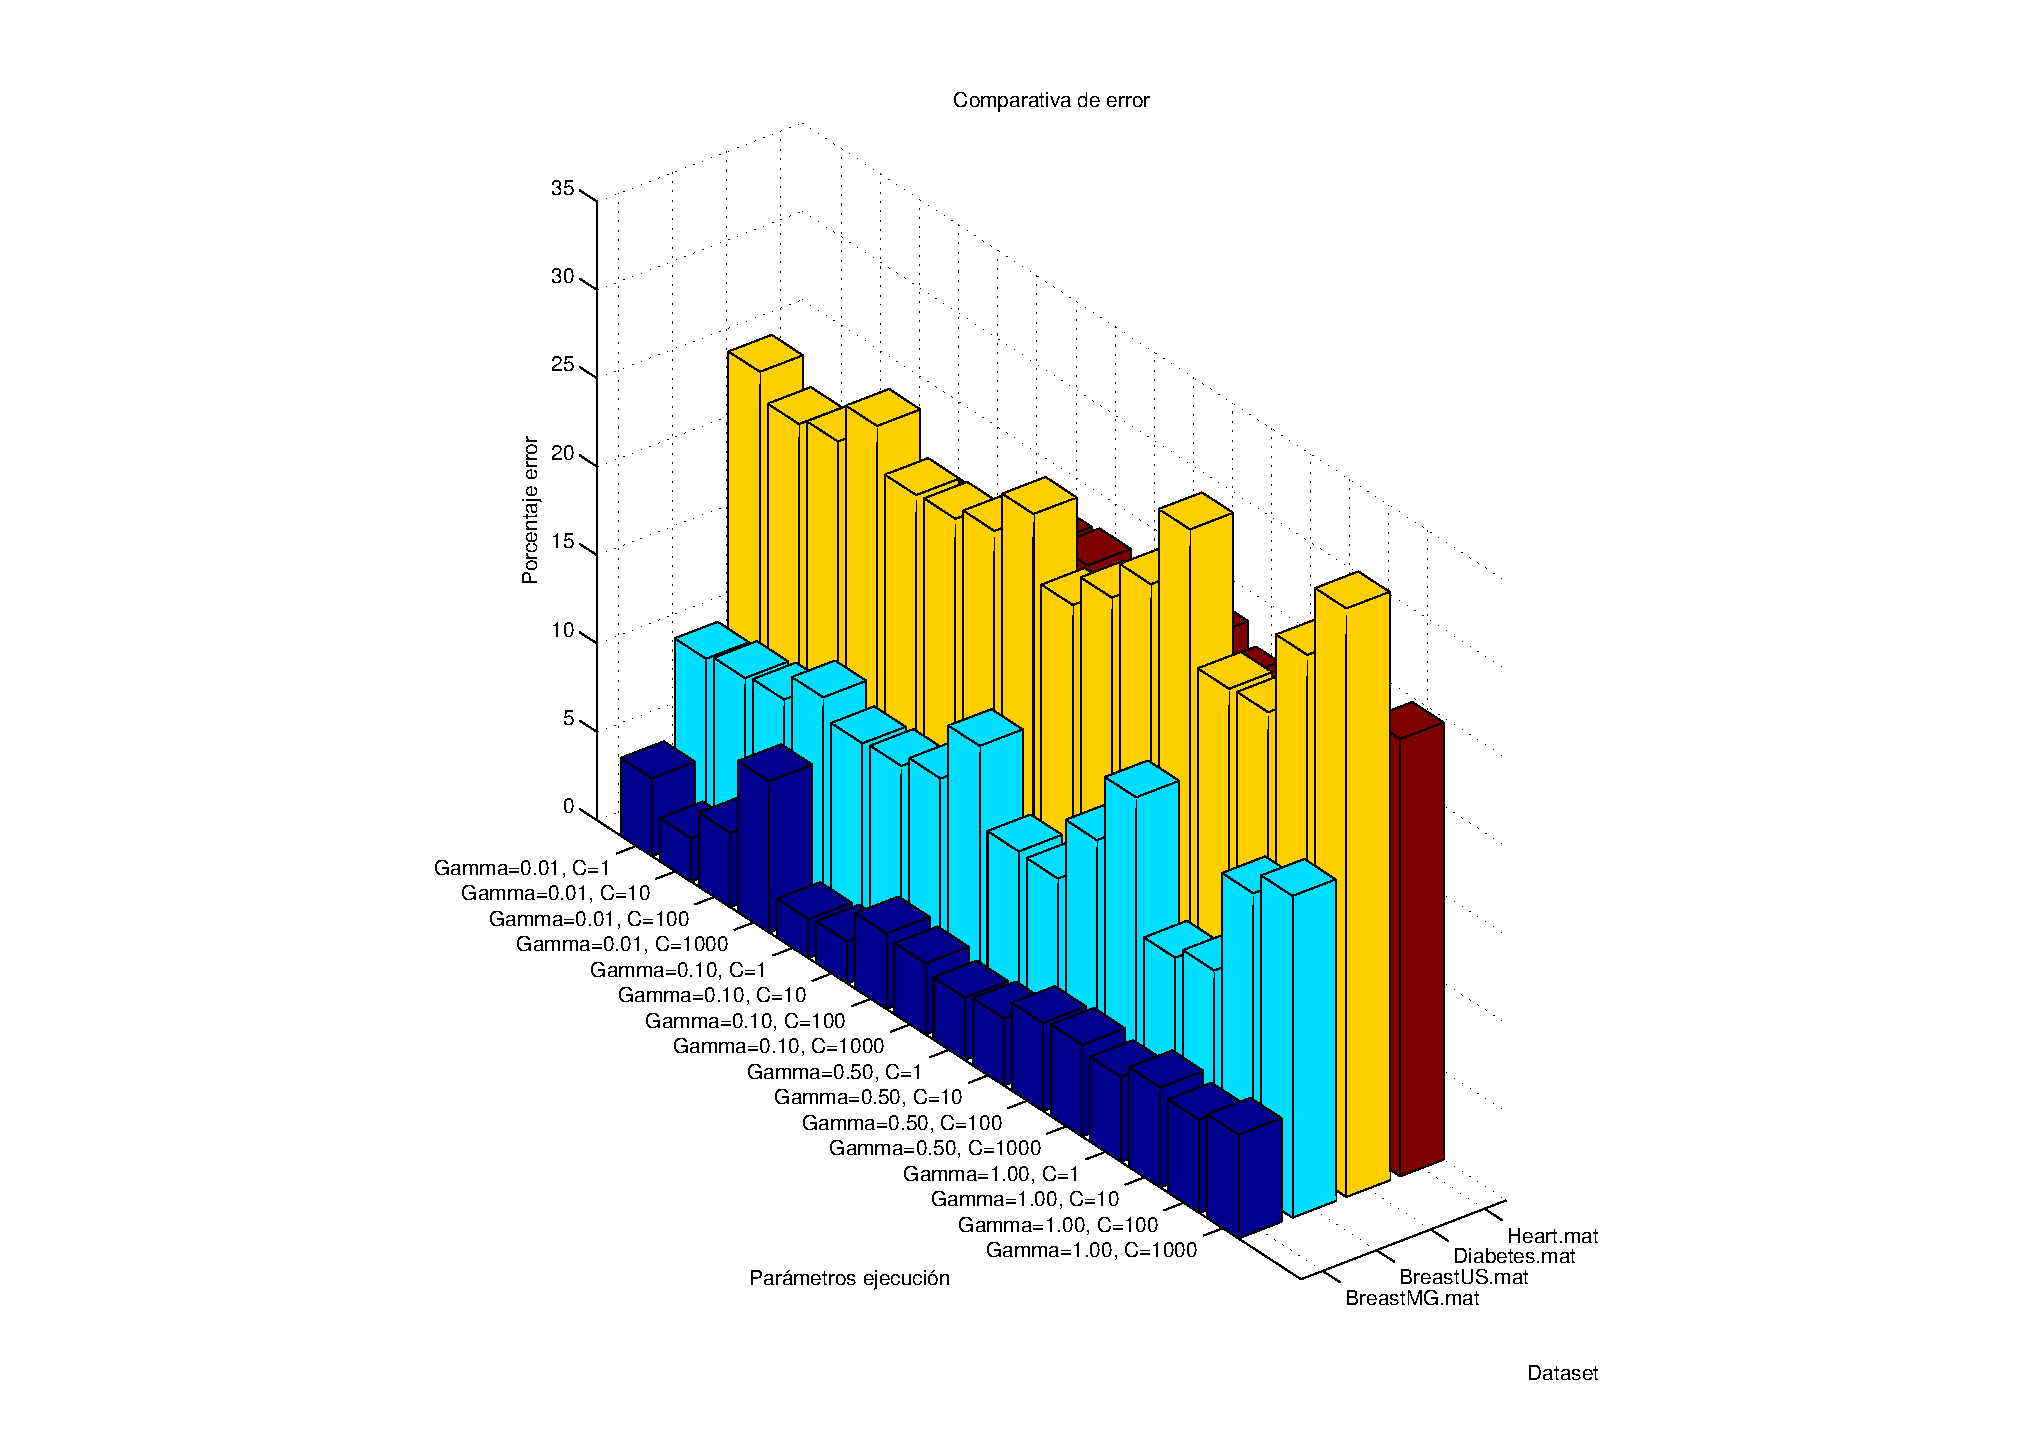
\includegraphics[width=\textwidth]{imagenes/rbf-error}
        \caption{Porcentajes de error obtenidos por la función kernel \emph{rbf}.}\label{fig:rbf-error}
\end{figure}


\begin{figure}
        \centering
        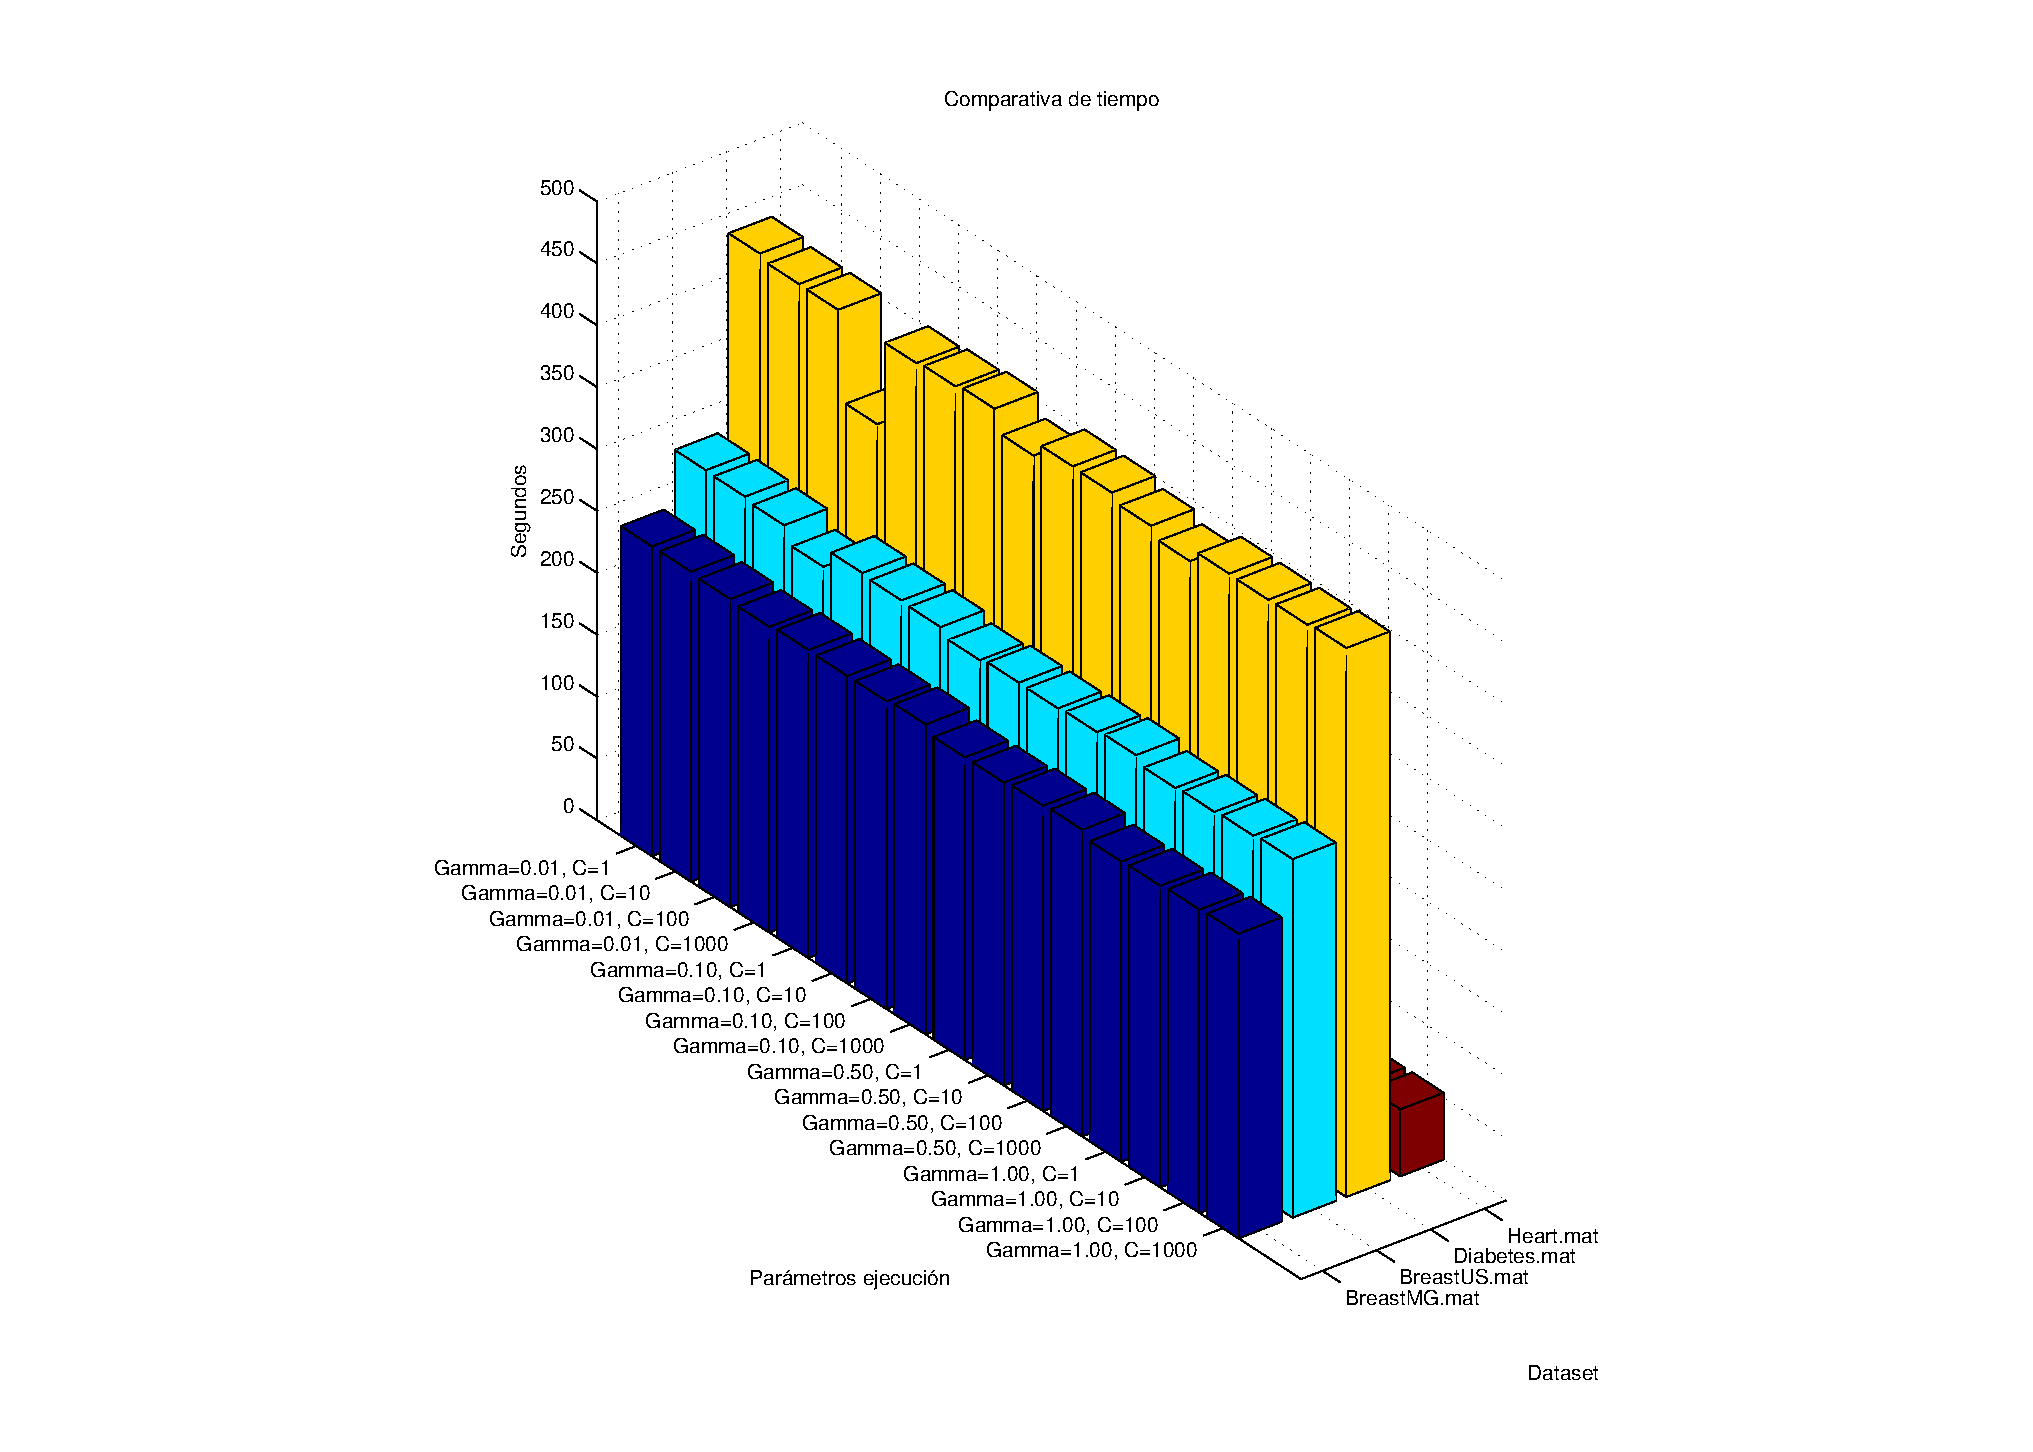
\includegraphics[width=\textwidth]{imagenes/rbf-time}
        \caption{Tiempos de ejecución obtenidos por la función kernel \emph{rbf}.}\label{fig:rbf-time}
\end{figure}

La ejecución de todo el experimento alcanzó los 30'458 segundos $\approx$ 8 horas.
Atendiendo a los mejores resultados de la ejecución de cada función kernel, tal como se muestra en la Tabla \ref{tbl:resultados-globales}, la función kernel \emph{rbf} obtiene los porcentajes de error más bajos.

\begin{table}[h]
\scriptsize
\centering
\begin{tabular}{@{}c|cc|cc|cc|cc@{}}
\toprule
\textbf{}  & \multicolumn{2}{c|}{\textbf{BreastMG}} & \multicolumn{2}{c|}{\textbf{BreastUS}} & \multicolumn{2}{c|}{\textbf{Diabetes}} & \multicolumn{2}{c}{\textbf{Heart}} \\
           & \emph{\% error}          & \emph{Parámetros}         & \emph{\% error}          & \emph{Parámetros}         & \emph{\% error}          & \emph{Parámetros}         & \emph{\% error}        & \emph{Parámetros}        \\ %\cmidrule{2-9}
Lineal     & 2.3719            & C=1                & 9.3794            & C=10               & 24.109            & C=10               & 17.324          & C=10              \\
Polinomial & 3.814             & O=2, C=1           & 11.29             & O=2,C=10           & 24.755            & O=2, C=1           & 23.337          & O=5, C=100        \\
rbf        & 2.2011            & $\gamma$=0.1, C=1          & 9.993             & $\gamma$=0.01, C=1         & 23.394            & $\gamma$=0.5, C=1          & 15.93           & $\gamma$=0.01, C=10      
\\ \bottomrule
\end{tabular}
\caption{Mejores resultados por dataset.}
\label{tbl:resultados-globales}
\end{table}

\section{Conclusiones}
El presente documento ha presentado los resultados obtenidos de la implementación de un clasificador \emph{SVM} utilizando las funciones kernel lineal, polinomial y \emph{rbf} utilizando diferentes valores para su cálculo.
Gracias al uso del \emph{truco} del kernel, los clasificadores lineales obtienen la posibilidad de trabajar con datos que en un inicio no son linealmente separables, pero que al ver aumentada su dimensionalidad podrían evidenciar algún grado de separación.

Tomando como base los datasets proporcionados y atendiendo a los mejores resultados en cada dataset por cada una de las funciones kernel implementadas, la función kernel \emph{rbf} obtiene los mejores resultados, con la excepción del caso del dataset \emph{BreastUS} en el que se ve superado por la función kernel lineal.
\end{document}